%%%%%%%%%%%%%%%%%%%%%%%%%%%%%%%%%%%%%%%%%
% Short Sectioned Assignment LaTeX Template Version 1.0 (5/5/12)
% This template has been downloaded from: http://www.LaTeXTemplates.com
% Original author:  Frits Wenneker (http://www.howtotex.com)
% License: CC BY-NC-SA 3.0 (http://creativecommons.org/licenses/by-nc-sa/3.0/)
%%%%%%%%%%%%%%%%%%%%%%%%%%%%%%%%%%%%%%%%%

%----------------------------------------------------------------------------------------
%	PACKAGES AND OTHER DOCUMENT CONFIGURATIONS
%----------------------------------------------------------------------------------------

\documentclass[paper=a4, fontsize=11pt]{scrartcl} % A4 paper and 11pt font size

% ---- Entrada y salida de texto -----

\usepackage[T1]{fontenc} % Use 8-bit encoding that has 256 glyphs
\usepackage[utf8]{inputenc}
%\usepackage{fourier} % Use the Adobe Utopia font for the document - comment this line to return to the LaTeX default

% ---- Idioma --------

\usepackage[spanish, es-tabla]{babel} % Selecciona el español para palabras introducidas automáticamente, p.ej. "septiembre" en la fecha y especifica que se use la palabra Tabla en vez de Cuadro

\usepackage{fancyhdr}

% ---- Otros paquetes ----

\usepackage{amsmath,amsfonts,amsthm} % Math packages
%\usepackage{graphics,graphicx, floatrow} %para incluir imágenes y notas en las imágenes
\usepackage{graphics,graphicx, float} %para incluir imágenes y colocarlas

% Para hacer tablas comlejas
%\usepackage{multirow}
%\usepackage{threeparttable}

%\usepackage{sectsty} % Allows customizing section commands
%\allsectionsfont{\centering \normalfont\scshape} % Make all sections centered, the default font and small caps

\usepackage{fancyhdr} % Custom headers and footers
\usepackage{url}
\usepackage{hyperref}
%\usepackage{hyperref}
\pagestyle{fancyplain} % Makes all pages in the document conform to the custom headers and footers
\fancyhead{} % No page header - if you want one, create it in the same way as the footers below
\fancyfoot[L]{} % Empty left footer
\fancyfoot[C]{} % Empty center footer
\fancyfoot[R]{\thepage} % Page numbering for right footer
\renewcommand{\headrulewidth}{0pt} % Remove header underlines
\renewcommand{\footrulewidth}{0pt} % Remove footer underlines
\setlength{\headheight}{13.6pt} % Customize the height of the header

\numberwithin{equation}{section} % Number equations within sections (i.e. 1.1, 1.2, 2.1, 2.2 instead of 1, 2, 3, 4)
\numberwithin{figure}{section} % Number figures within sections (i.e. 1.1, 1.2, 2.1, 2.2 instead of 1, 2, 3, 4)
\numberwithin{table}{section} % Number tables within sections (i.e. 1.1, 1.2, 2.1, 2.2 instead of 1, 2, 3, 4)

\setlength\parindent{0pt} % Removes all indentation from paragraphs - comment this line for an assignment with lots of text

\newcommand{\horrule}[1]{\rule{\linewidth}{#1}} % Create horizontal rule command with 1 argument of height

\usepackage{booktabs}




%----------------------------------------------------------------------------------------
%	TÍTULO Y DATOS DEL ALUMNO
%----------------------------------------------------------------------------------------

\title{	
\normalfont \normalsize 
\textsc{{\bf Técnicas de Sistemas Inteligentes (2014-2015)} \\ Grado en Ingeniería Informática \\ Universidad de Granada} \\ [25pt] % Your university, school and/or department name(s)
\horrule{0.5pt} \\[0.4cm] % Thin top horizontal rule
\huge  Práctica 3.2 - Dominios y problemas de planificación HTN. \\ % The assignment title
\horrule{2pt} \\[0.5cm] % Thick bottom horizontal rule
}

\author{Ignacio Martín Requena} % Nombre y apellidos

\date{\normalsize\today} % Incluye la fecha actual

%----------------------------------------------------------------------------------------
% DOCUMENTO
%----------------------------------------------------------------------------------------
\usepackage{graphicx}
\usepackage{listings}
\usepackage{color}
\definecolor{gray97}{gray}{.97}
\definecolor{gray75}{gray}{.75}
\definecolor{gray45}{gray}{.45}
 

\lstset{ frame=Ltb,
     framerule=0pt,
     aboveskip=0.5cm,
     framextopmargin=3pt,
     framexbottommargin=3pt,
     framexleftmargin=0.2cm,
     framesep=0pt,
     rulesep=.4pt,
     backgroundcolor=\color{gray97},
     rulesepcolor=\color{black},
     %
     stringstyle=\ttfamily,
     showstringspaces = false,
     basicstyle=\small\ttfamily,
     commentstyle=\color{gray45},
     keywordstyle=\bfseries,
     %
     numbers=left,
     numbersep=15pt,
     numberstyle=\tiny,
     numberfirstline = false,
     breaklines=true,
   }
 


\lstdefinestyle{consola}
   {basicstyle=\scriptsize\bf\ttfamily,
    backgroundcolor=\color{gray75},
   }
 
\lstdefinestyle{C}
   {language=C,
   }



\begin{document}

\maketitle % Muestra el Título

\newpage %inserta un salto de página

\tableofcontents % para generar el índice de contenidos

\listoffigures

%\listoftables

\newpage




%----------------------------------------------------------------------------------------
%	Cuestion 1
%----------------------------------------------------------------------------------------

\section{Ejercicio 0}
Se puede comprobar como con el dominio \texttt{zenotravel-V00.pddl} y el problema  \texttt{problema-zeno-0.pddl} entregado por el profesor el planificador HTN-PDDL resuelve el problema:

\begin{figure}[h]
\centering
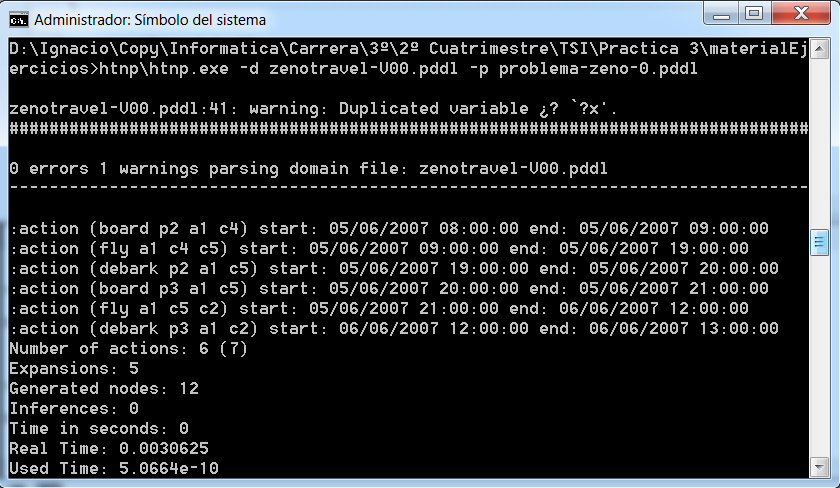
\includegraphics[width=0.9\linewidth]{p0}
\caption{Ejecución de HTN para el problema 0}
\label{fig:p0}
\end{figure}

Como podemos ver en la \textbf{Figura \ref{fig:p0}} HTN nos devuelve el plan a seguir para resolver el problema introducido.


%----------------------------------------------------------------------------------------
%	Cuestion 2
%----------------------------------------------------------------------------------------
\section{Ejercicio 1}

Ahora se pide modificar el dominio anterior para poder resolver el problema de transportar 3 personas (inicialmente en las ciudades C1, C2 y C3) a la ciudad C5, considerando que el avión está en la ciudad C4. Se asume al igual que en el problema ejemplo que no hay restricciones de fuel.\\

Si realizamos una ejecución directa, el resultado es:

\begin{figure}[H]
\centering
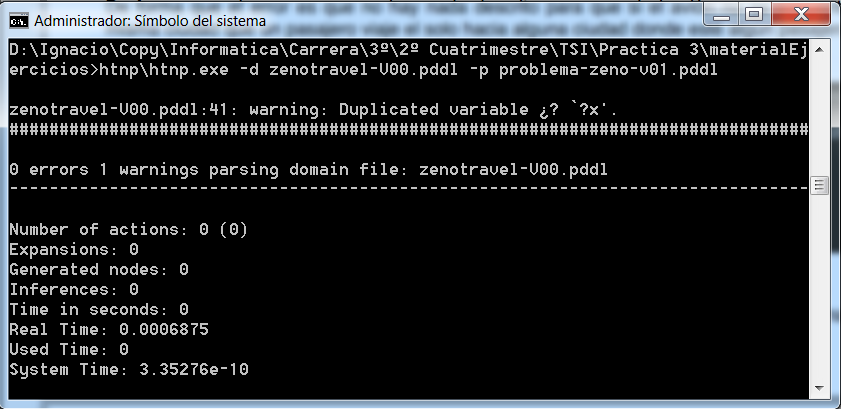
\includegraphics[width=0.7\linewidth]{p11}
\caption{Ejecución de HTN para el problema 1 sin modificar el dominio}
\label{fig:p1}
\end{figure}

Como podemos ver, ahora HTN no es capaz de encontrar un plan para resolver el problema. Si analizamos el dominio con detenimiento nos damos cuenta de que no hay nada descrito que resuelva el hecho de que si el aión no está en la misma ciudad que un pasajero este sea capaz de ir hacia alguna ciudad donde esté algún otro pasajero.\\

Para resolver este problema, en el dominio, incluimos lo siguiente:



	
	\begin{lstlisting}[language=SH]
  (:method Case3 ;si no esta en la ciudad destino, y avion y persona no estan en la misma ciudad
  :precondition (and (at ?p - person ?c1 - city) (at ?a - aircraft ?c2 - city))
  
  :tasks ( 
	  (mover-avion ?a ?c2 ?c1)
	  (board ?p ?a ?c1)
	  (mover-avion ?a ?c1 ?c)
	  (debark ?p ?a ?c )))

	\end{lstlisting}

Simplemente hemos añadido otra precondición para realizar la acción de mover el avión a la ciudad donde está la persona y en la lista de tareas añadida la acción de desplazar el avión hasta la localización de la persona que no puede acceder a el.\\	
	
De esta forma podemos comprobar como ya si encontramos un plan que resuelva el problema:

\begin{figure}[H]
	\centering
	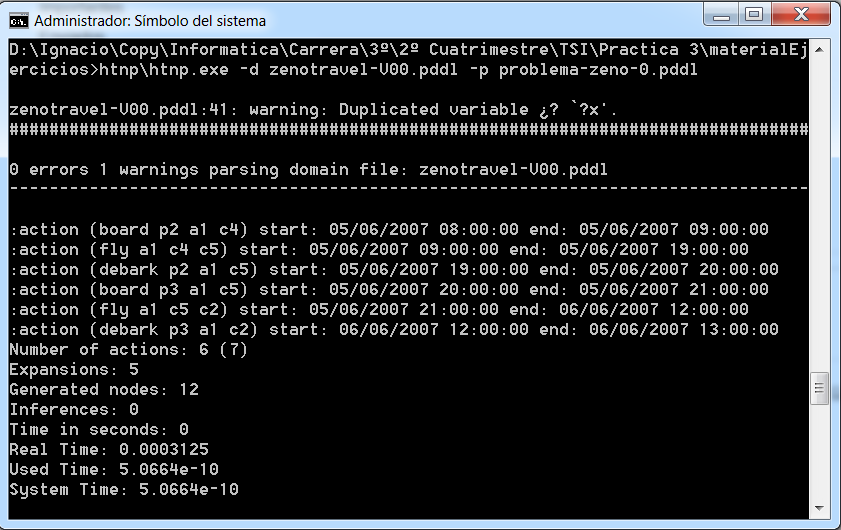
\includegraphics[width=0.7\linewidth]{p12}
	\caption{Ejecución de HTN para el problema 1 con dominio modificado}
	\label{fig:p12}
\end{figure}
		
\section{Ejercicio 2}

Ahora nuestro problema consiste en asumir que hay restricciones de fuel. El fuel inicial del avión es de 200 y la capacidad total de 300.\\

En primer lugar ejecutaremos el problema para el dominio sin modificar y observaremos los resultados que HTN nos muestra: 

\begin{figure}[H]
	\centering
	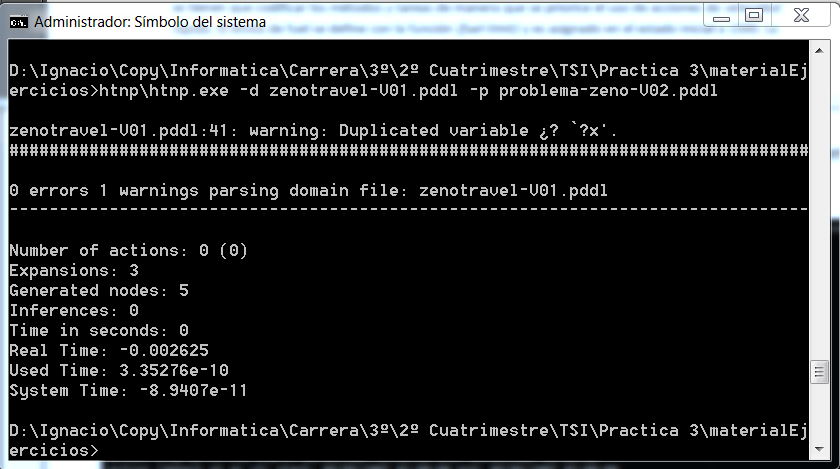
\includegraphics[width=0.7\linewidth]{p21}
	\caption{Ejecución de HTN para el problema 2 con dominio no modificado}
	\label{fig:p21}
\end{figure}

Como podemos ver, el resultado de la ejecución es similar al obtenido en la \textbf{Figura \ref{fig:p0}}, sin acciones ni errores que nos indiquen donde se haya el error.\\

Ahora, como cabe esperar, el problema radica en que no se posee de acciones para realizar el repostaje de un avión. Para solucionarlo añadiremos el siguiente método a nuestro dominio:

	\begin{lstlisting}[language=SH]
  (:method no-hay-fuel
	  :precondition (not(hay-fuel ?a ?c1 ?c2))
	  :tasks (
		  (refuel ?a ?c1)
		  (fly ?a ?c1 ?c2)
	  )
  )

	
	\end{lstlisting}

Este método se escogerá cuando no haya fuel suficiente. En primer lugar se repostará el avión para, a continuación, continuar con la marcha del vuelo.\\

Ahora si, HTN encuentra un plan para nuestro problema:\\

\begin{figure}[H]
	\centering
	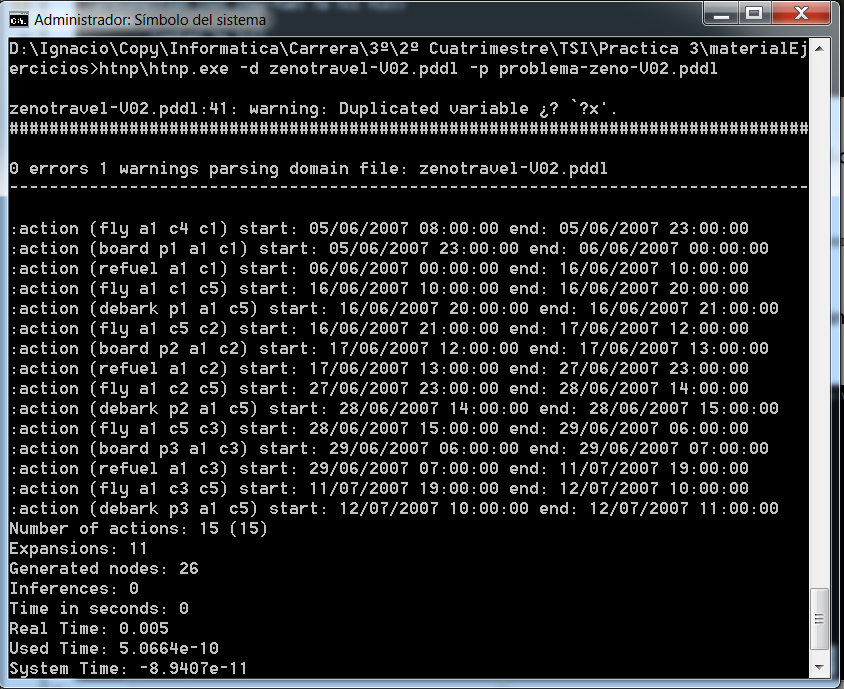
\includegraphics[width=0.8\linewidth]{p22}
	\caption{Ejecución de HTN para el problema 2 con dominio correcto}
	\label{fig:p22}
\end{figure}

\section{Ejercicio 3}
Por último, para este conjunto de ejercicios, ahora se pide que se consideren acciones de vuelo lento y
rápido para tratar de transportar las personas lo más rápido posible con un límite de fuel.\\

Como siempre, en primer lugar ejecutaremos nuestro dominio sobre el problema a resolver:\\

\begin{figure}[H]
	\centering
	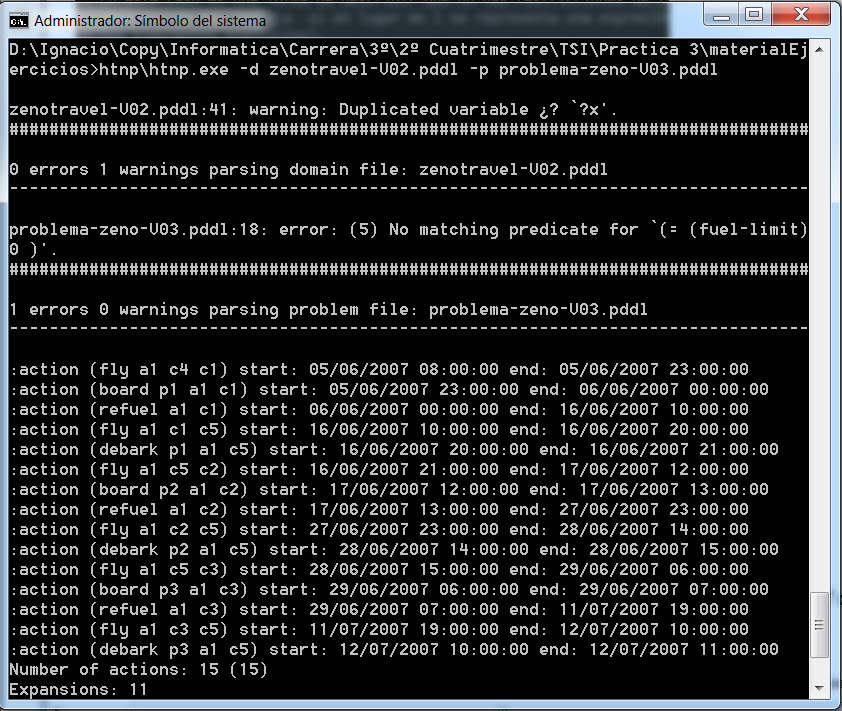
\includegraphics[width=0.8\linewidth]{p31}
	\caption{Ejecución de HTN para el problema 3 con dominio no modificado}
	\label{fig:p31}
\end{figure}

En este caso si podemos encontrar pero sin tener definidas las acciones de vuelo lento y vuelo rápido. Para cumplir estos requisitos modificaremos lo siguiente:
\newpage
\begin{itemize}
	\item En primer lugar se ha modificado el fichero ``Primitivas-ZenoTravel.pddl'' para añadirle las primitivas que posee el archivo ``Primitivas-ZenoTravel-Pretty'' proporcionado.
	
	\item Se han añadido dos nuevos predicados para representar el gasto rápido y lento de fuel:
	
	\begin{lstlisting}[language=SH]
(:predicates (at ?x - (either person aircraft) ?c - city)
	(in ?p - person ?a - aircraft)
	(different ?x ?y) (igual ?x ?y)
	(hay-fuel-rapido ?a ?c1 ?c2) ; gasto rapido de fuel
	(hay-fuel-lento ?a ?c1 ?c2) ;gasto lento de fuel
	)
	\end{lstlisting}
	
	\item Se ha añadido una nueva función para controlar el límite de fuel llamada \texttt{(fuel-limit)}
	
	\item Se ha cambiado el derivado original por dos nuevos, uno para el gasto rápido de fuel y otro para el gasto lento:
	
	\begin{lstlisting}[language=SH]
(:derived 

	(hay-fuel-rapido ?a - aircraft ?c1 - city ?c2 - city)
	(> (fuel ?a) (* distance ?c1 ?c2) (fast-burn ?a))
)

(:derived 

	(hay-fuel-lento ?a - aircraft ?c1 - city ?c2 - city)
	(> (fuel ?a) (* distance ?c1 ?c2) (slow-burn ?a))
)
	\end{lstlisting}
	
	\item Se han cambiado los métodos de la tarea de mover-avion, conservando la filosofía de tener dos métodos que comprueban si hay o no fuel, aunque, en este caso diferenciando entre si se está en un estado lento o rápido de vuelo:
	
\begin{lstlisting}[language=SH]
(:task mover-avion
	:parameters (?a - aircraft ?c1 - city ?c2 -city)
	
	(:method fuel-suficiente-rapido 
	 :precondition (and(hay-fuel-rapido ?a ?c1 ?c2)(>(fuel-limit)(total-fuel-used)))
	 
	 :tasks (
	    (zoom ?a ?c1 ?c2)
	  )
	)
	
	(:method no-hay-fuel-rapido 
	 :precondition (and (not(hay-fuel-rapido ?a ?c1 ?c2))(>(fuel-limit)(total-fuel-used)))
	 
	 :tasks (
	   (refuel ?a ?c1)
	   (zoom ?a ?c1 ?c2)
	 )
	)
	
	
	
	(:method fuel-suficiente-lento 
	 :precondition (and(hay-fuel-lento ?a ?c1 ?c2)(>(fuel-limit)(total-fuel-used)))
	 
	 :tasks (
	   (fly ?a ?c1 ?c2)
	 )
	)
	
	(:method no-hay-fuel-lento 
	 :precondition (and (not(hay-fuel-lento ?a ?c1 ?c2))(>(fuel-limit)(total-fuel-used)))
	 
	 :tasks (
		(refuel ?a ?c1)
		(fly ?a ?c1 ?c2)
	 )
	)
)

\end{lstlisting}

Una vez realizadas estas modificaciones podemos ver como HTN ya si nos muestra un plan correcto:


\begin{figure}[H]
	\centering
	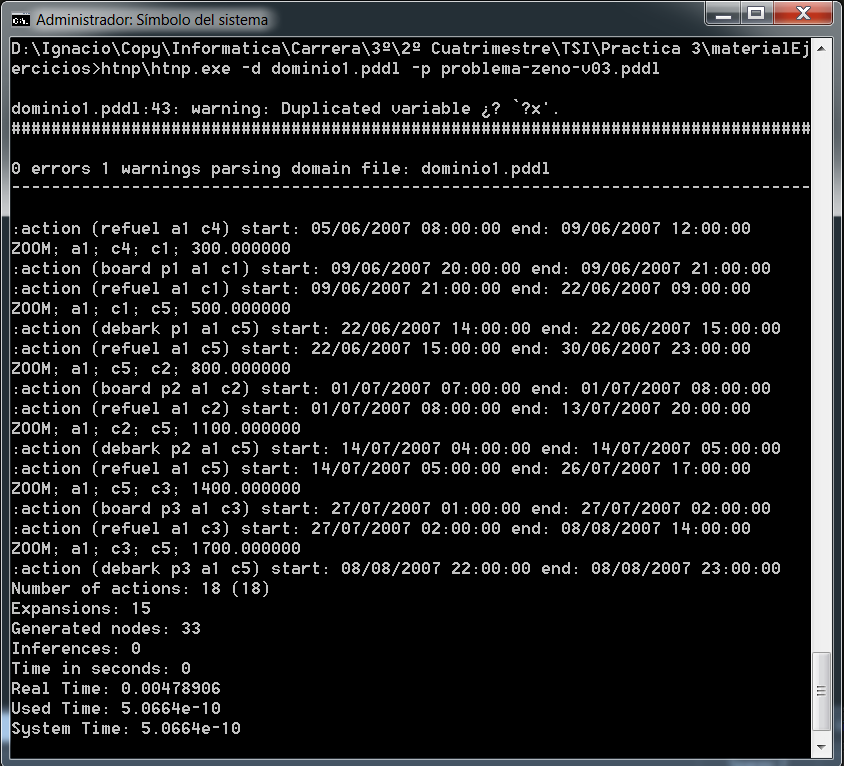
\includegraphics[width=0.8\linewidth]{p32}
	\caption{Ejecución de HTN para el problema 3 con dominio no modificado}
	\label{fig:p32}
\end{figure}
	
\end{itemize}

\newpage
\section{Ejercicio 4}

Para este ejercicio se pide que se extienda el problema anterior con el fin de controlar la entrada de pasajeros a un avión (embarque/desembarque).

Las modificaciones realizadas sobre el código de partida de forma esquemática (debido al número de páginas) han sido:

\begin{itemize}
	\item Se han añadido los siguientes \textbf{predicados}:
	
	\begin{lstlisting}[language=SH]
(embarcar ?a ?p)
(desembarcar ?a ?p)
(destino ?p - person ?c1 - city)
	             
	 \end{lstlisting}
	
	\item \textbf{Literales derivados}: se han añadido tres literales derivados, uno para hacer iguales las distancias entre dos ciudades alternando el orden de escritura y otros dos para controlar si se supera la capacidad del avión o si está vacío
	
	\begin{lstlisting}[language=SH]
(:derived 

(distance ?c1 - city ?c2 - city)
(= (distance ?c2 - city ?c1 - city) (distance ?c1 - city ?c2 - city) )
)

(:derived 

(embarcar ?a - aircraft ?p - person)
(< (capacity ?a) (+ (capacity ?a) 1))
)

(:derived 

(desembarcar ?a - aircraft ?p - person)
(< (capacity ?a) (- (capacity ?a) 1))
)
		\end{lstlisting}
	
	\item Se ha modificado la tarea \texttt{tansport-person} para representar la acción de embarcar y desembarcar un pasajero del avión
	
		
	\item Se han creado dos nuevas \textbf{tareas compuestas} para que puedan embarcarse varios pasajeros en un avión. Con respecto a este apartado, decir que no se ha logrado acabar de implementar el dominio debido a que no he conseguido solucionar el error de que HTN no reconocía las tareas de embarque y desembarque como acciones a realizar. 
	
	Tras hacer uso con el debugger (opción display -d-) se ha conseguido acotar el error al siguiente:
	
	
	\begin{figure}[H]
		\centering
		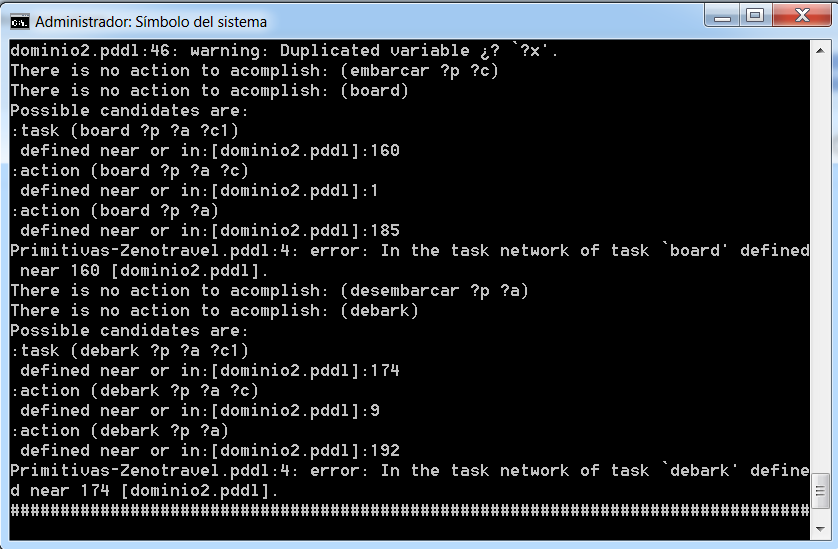
\includegraphics[width=0.7\linewidth]{p41}
		\caption{Ejecución de HTN para el problema 2 con dominio no modificado}
		\label{fig:p21}
	\end{figure}
	
	Como no se ha conseguido finalizar el dominio requerido para resolver el problema no se ha podido probar el problema implementado. Este problema, basado en las distancias entre aeropuertos de España, posee dos aviones diferentes que embarcan y desembarcan en aeropuertos de la forma mas eficiente posible (consumiendo el menor numero de fuel).
	
	Debido a la gran extensión del problema, ya que hay que especificar todas las distancias entre todos los aeropuertos, no se ha incluido en este documento su implementación, si no que se encuentra adjunto, en la carpeta ``Archivos''.
	
	
	
	

\end{itemize}

\section{Aclacación}

El fichero ha superado las 5 páginas permitidas debido a la necesidad de introducción parcial del código desarrollado, si se suprime este la exigencia de la extensión se respeta.

\end{document}